%%
%% methodology.tex
\forcecommand{\thesec}{Methodology}
\section{\thesec}
\label{sec:methodology}
%%


%%
\forcecommand{\thesubsec}{Smoothed Particle Hydrodynamics}
%%
\begin{frame}{\thesec}{\thesubsec}
  \vspace*{-2\baselineskip}
  \begin{block}{SPH overview:}
    \begin{columns}
      \begin{column}{0.9\paperwidth}
        \begin{itemize}
          \item{
            fully Lagrangian, mesh-free method for modeling continuous media
          }
		  \item{ 
		    models continua as collections of \alert{particles}
		    \begin{itemize}
		        \item{ each particle has a fixed mass }
		        \item{ 
		          particle motion is governed by Classical Mechanical laws of motion (Newton's Second Law)
		        }
		        \item{
		          particles have thermodynamic properties (temperature, density, pressure, etc.)
		        }
		        \item{
		          not point particles---should be thought of as large ensembles of microscopic particles (Statistical Mechanics) or as material fluid elements (Continuum Mechanics)
		        }
		    \end{itemize}
		  }
        \end{itemize}
      \end{column}
    \end{columns}
  \end{block}
\end{frame}

\begin{frame}{\thesec}{\thesubsec}
  \vspace*{-2.1\baselineskip}
  \begin{figure}
    \centering
    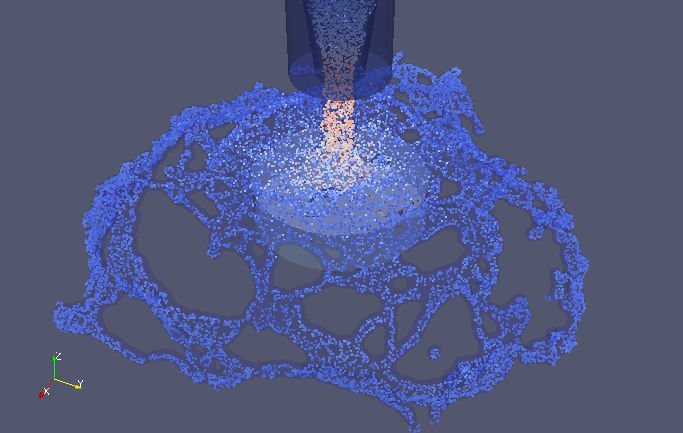
\includegraphics[width=0.9\textwidth]{img/ren_marshall_close.png}
  \end{figure}
\end{frame}

\begin{frame}{\thesec}{\thesubsec}
  \vspace*{-2\baselineskip}
  \begin{itemize}
    \item{
      SPH is a popular method for studying violent hydrodynamic flows, particularly those involving a free surface with large deformations and fragmentation
      \begin{itemize}
        \item{
          validated in tests involving wave breaking, wave-structure interaction, and, of particular interest to the present work, the free surface flow around a moving ship
        }
      \end{itemize}
    }
    \item{
      SPH is well suited to problems involving enormous variations in the relevant length scales
      \begin{itemize}
        \item{
          examples exist in astrophysical literature illustrating the ability of SPH to capture phenomena on length scales varying across several orders of magnitude
        }
      \end{itemize}
    }
  \end{itemize}
\end{frame}

\begin{frame}{\thesec}{\thesubsec}
  \vspace*{-2\baselineskip}
  \begin{itemize}
    \item{
      almost all applications of SPH to modeling wave-structure interaction and ship hydrodynamics focus on wave heights and profiles, and loading of structures
    }
    \vspace*{2\baselineskip}
    \item{
      very little work exists regarding the application of SPH to breakup phenomena
      \begin{itemize}
        \item{
          ability of SPH and its variants to accurately model breakup phenomena must be validated!
        } 
      \end{itemize}
    }
  \end{itemize}
\end{frame}

%%
\forcecommand{\thesubsec}{Focus of Current Work}
%%
\begin{frame}{\thesec}{\thesubsec}
  \vspace*{-2\baselineskip}
  \begin{itemize}
    \item{
	  simulate small-scale (i.e.~lab scale) experiments to determine applicability of SPH to larger-scale problems
	  \begin{itemize}
	    \item{
	      spray generation due to the oblique impact of a jet/sheet of water against a solid surface is closely related to the process of wave spray generation
	    }
	  \end{itemize}
	}
	\vspace*{\baselineskip}
	\item{
	  experimental data exists which can be used to validate the code
	  \begin{itemize}
	    \item{e.g.~Ren and Marshall, 2014}
	  \end{itemize}
	}
  \end{itemize}
\end{frame}

%%
%% current jet impingement
\begin{frame}{\thesec}{Ren and Marshall 2014 Experiment}
  \vspace*{-\baselineskip}
  \begin{columns}
    \begin{column}{\paperwidth}
      \begin{figure}
        \centering
        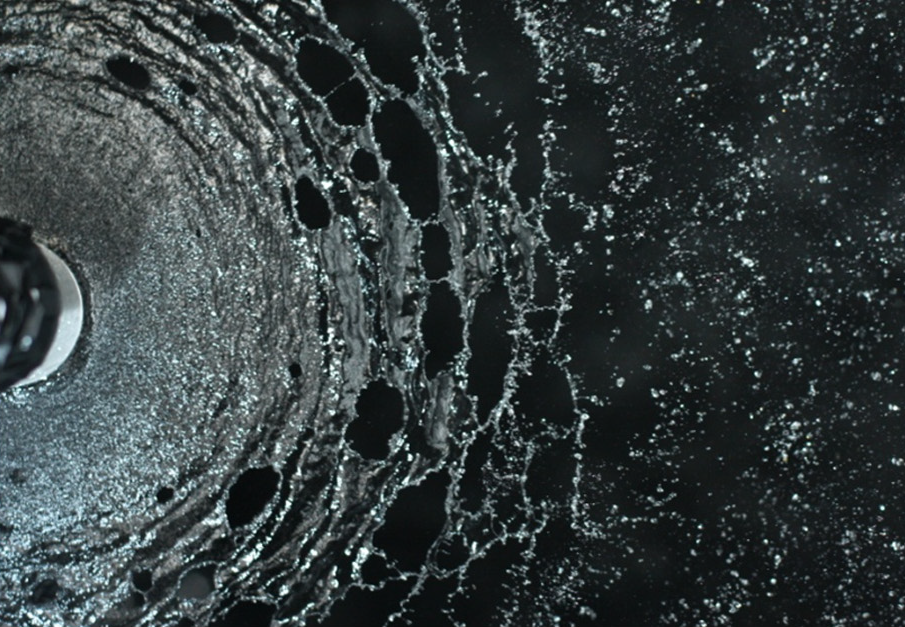
\includegraphics[width=\paperwidth]{img/flappingSheetBreakup2.png}
        \caption{From Ren and Marshall, 2014}
        \label{fig:ren_marshall_breakup_15300}
      \end{figure}
    \end{column}
  \end{columns}
\end{frame}

\begin{frame}{\thesec}{Ren and Marshall 2014 Experiment}
  \vspace*{-2.1\baselineskip}
  \begin{columns}
    \begin{column}{0.45\textwidth}
      \begin{figure}
        \centering
        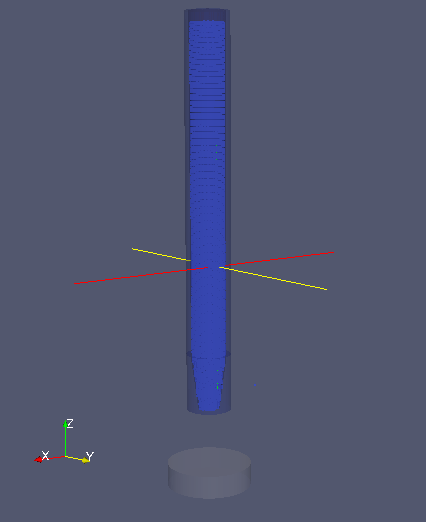
\includegraphics[width=\textwidth]{img/ren_marshall_start.png}
      \end{figure}
    \end{column}
    \begin{column}{0.45\textwidth}
      \begin{figure}
        \centering
        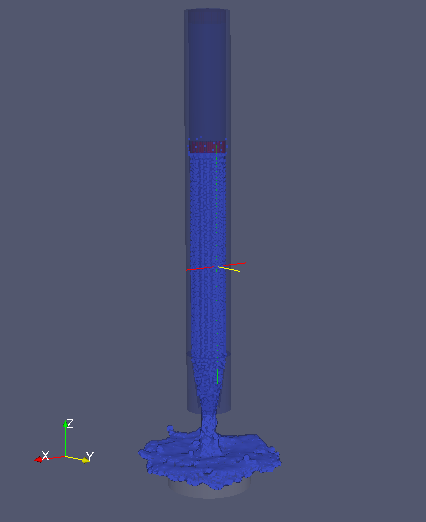
\includegraphics[width=\textwidth]{img/ren_marshall_mid.png}
      \end{figure}
    \end{column}
  \end{columns}
\end{frame}
%% M. Sullivan. June, 2016